\documentclass[twocolumn]{article}
\usepackage{graphicx}
\usepackage{fullpage}
\usepackage{comment}
\usepackage{amsmath}

\usepackage{listings}
\usepackage{courier}
\usepackage{xcolor}
\definecolor{commentsColor}{rgb}{0.497495, 0.497587, 0.497464}
\definecolor{keywordsColor}{rgb}{0.000000, 0.000000, 0.635294}
\definecolor{stringColor}{rgb}{0.558215, 0.000000, 0.135316}
\lstset{
  basicstyle=\ttfamily\small,                   % the size of the fonts that are used for the code
  breakatwhitespace=false,                      % sets if automatic breaks should only happen at whitespace
  breaklines=true,                              % sets automatic line breaking
  frame=tb,                                     % adds a frame around the code
  commentstyle=\color{commentsColor}\textit,    % comment style
  keywordstyle=\color{keywordsColor}\bfseries,  % keyword style
  stringstyle=\color{stringColor},              % string literal style
  numbers=left,                                 % where to put the line-numbers; possible values are (none, left, right)
  numbersep=5pt,                                % how far the line-numbers are from the code
  numberstyle=\tiny\color{commentsColor},       % the style that is used for the line-numbers
  showstringspaces=false,                       % underline spaces within strings only
  tabsize=2,                                    % sets default tabsize to 2 spaces
  language=C
}




\title{Analysis of "quick and dirty" implementation of exponential function}
\author{Christian Norre}
\date{}
\begin{document}
\maketitle

\begin{abstract}
We show some basic capabilities of \LaTeX: math, figures,
references, citations, and sections.
\end{abstract}

\section{The exponential function}
The exponential function is defined as the solution to the differential equation:
\begin{align}
\frac{d\,y(x)}{dx} = y(x)\quad,\quad y(0)=1\;.
\end{align}
A common way of working with it is by its Taylor expansion:
\begin{align} 
\exp(x) = \sum_{n=0}^\infty \frac{x^n}{n!}\,, \label{eq:sum}
\end{align}
where, when we implement it in computers, we have to use a finite number of terms.

\section{The implementation}

\begin{lstlisting}
double ex(double x){
	if(x<0)return 1/ex(-x);
	if(x>1./8)return pow(ex(x/2),2);
	return 1+x*(1+x/2*(1+x/3*(1+x/4*(1+x/5*(1+x/6*(1+x/7*(1+x/8*(1+x/9*(1+x/10)))))))));
}
\end{lstlisting}

Line 2 of the code is just a property of the exponential function $\exp(-x)=1/\exp(x)$, and so is the third line $\exp(x)=(\exp(x/2))^2$.

Line 4 is more complicated, but when multiplying out the parantheses, one acquires the first 10 terms of the Taylor series as we know them from the sum (equation \ref{eq:sum}).

Other than the fact that it looks stange, there is no reason why this implementation shouldn't work. A plot of this function can be seen in figure \ref{fig:exp}. A more enlightening comparison would be to plot the difference between ex(x) and a conventional $\exp(x)$ as seen in figure \ref{fig:exp_diff}. The exponential in math.h is naturally also an approximation with finite terms, but we trust that this implementation is sufficiently sophisticated to provide a good comparison to the true exponential function. The difference is rather small, so I conclude that this is a good implementation of the exponential function.

\begin{comment}
	\begin{figure}[h]
\input{fig-gpl.tex}
\caption{Nemes formula~(\ref{eq:nemes}) via gnuplot "latex" terminal.}
\label{fig:gpl}
	\end{figure}
\end{comment}


	\begin{figure}[h]
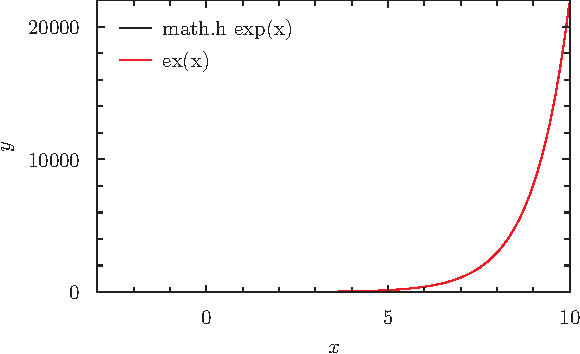
\includegraphics[width=\columnwidth]{exp_pyx.pdf}
\caption{Plot of this implementation of the exponential function along with the math.h implementation.}
\label{fig:exp}
	\end{figure}
	
		\begin{figure}[h]
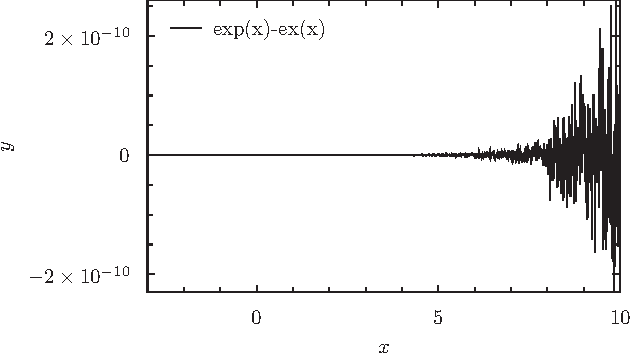
\includegraphics[width=\columnwidth]{exp_diff_pyx.pdf}
\caption{Plot of the difference between the implementations.}
\label{fig:exp_diff}
	\end{figure}
	
	
\section{Why}
The purpose of line 2 is to make sure we only work with positive numbers, as a negative number would result in a negative sign in every other term. Since this is an identity of the exponential function, we will not lose any accuracy by insisting on using positive numbers, but we gain increase precision in each operation, as differences are lossy.

Line 3 looks stange, but we must remember that a Taylor series does not converge uniformly. It converges the fastest near the evaluation point of the series (around $x=0$ for equation \ref{eq:sum}). This line utilises another identity of the exponential function to make sure that we actually only calculate the function when x is sufficiently small. The tradeoff is that we lose some precision when we square the result a couple of times to arrive at the desired result. But this loss in precision is much less that the loss which comes from evaluating the series far $x=0$.

The purpose of the way line 4 is written is that there are far fewer multiplication operations, and each of theses multiplications are acting on numbers of approximately the same order of magnitude. We have seen in previous exercises that doing math with large and small numbers at the same time is lossy. To check the effect of each of these choices, i have plotted the difference of ex(x) to more naive implementations in figure \ref{fig:exp_naive}. 

It is interesting to note that longsum(x) seems to make no difference in result (difference 0). This might be because the compiler is very smart and actually does the same thing no matter how I write it. For negative numbers, neg(x) is dominant, and for positive numbers, nohalf(x) is dominant.

\begin{figure}[h]
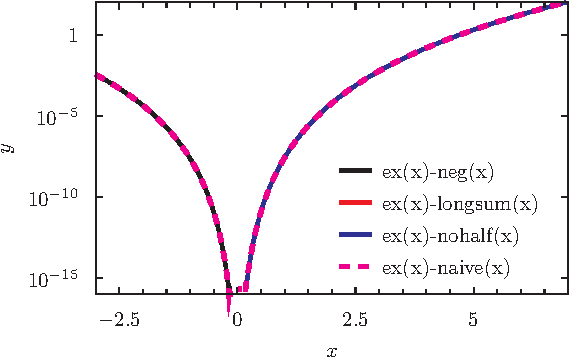
\includegraphics[width=\columnwidth]{exp_other.pdf}
\caption{Comparison between ex(x) and other naive implementations. neg(x) is where the negative check is removed. longsum(x) is using the conventional Taylor terms. nohalf(x) is not casting x to smaller values before calculating. naive(x) is all of the above.}
\label{fig:exp_naive}
	\end{figure}
	
	
	
\section{Complex equivalent}

\begin{lstlisting}
double complex cex(double complex z){
	double radius = ex(creal(z));
	return radius*(cos(cimag(z)) + I*sin(cimag(z)));
}
\end{lstlisting}

It might be cheating to use cos and sin, but i cant immediately see how else to do it. 

\end{document}
